\section{Tensors}
Tensors are algebraic objects that extend the concept of scalars, vectors, and matrices to higher dimensions and can be interpreted as a multi-dimensional array. The number of dimensions is usually called the ``rank'' or ``order'' of a tensor. A scalar, for example, can represent a zero-order tensor, a vector a first-order tensor, and a matrix a second-order tensor. Higher-order tensors have multiple dimensions. 
Each of these dimensions of a tensor is represented by an index. 
A tensor of order $ n $ can be written as $ T_{i_1 i_2 \dots i_n} $, where each index $ i_k $ runs over a certain range.
The size of a tensor is determined by the product of the values of each index’s range.

\section{Tensor Contractions}
\noindent Tensor contraction is an operation that reduces the order of one or more tensors by summing over their shared indices. It generalizes the concept of matrix multiplication, where summation occurs over a shared index. \\
For example, for matrices $A\in \mathbb{R}^{m\times p}$ and $B\in \mathbb{R}^{p\times n}$ , the result is a new matrix $C\in \mathbb{R}^{m\times n}$, computed as:
$$
C_{ij} = \sum_{k} A_{ik} B_{kj}
$$

\noindent For higher order tensors, the idea can be extended as follows: Let $T\in \mathbb{R}^{i_1\times ... \times i_p\times k_1 \times ... \times k_r}$ and $S\in \mathbb{R}^{k_1 \times ... \times k_r\times j_1 \times ... \times j_q}$. Then,

$$
C_{i_1, \dots, i_p, j_1, \dots, j_q} = \sum_{k_1, \dots, k_r} T_{i_1, \dots, i_p, k_1, \dots, k_r} S_{k_1, \dots, k_r, j_1, \dots, j_q}
$$

\noindent where the indices $ k_1, \dots, k_r $ are summed over, reducing the total number of dimensions in the resulting tensor $ C $.

\section{Tensor Networks}
A tensor network represents a complex tensor expression as a graph. Each tensor is represented by a node, and the indices of the tensors are represented by edges. If two tensors share an index, that index is contracted, and an edge connects the two nodes. Tensor networks where more than two tensors share the same index are called ``hypernetworks''. 

\begin{figure}
\begin{center}
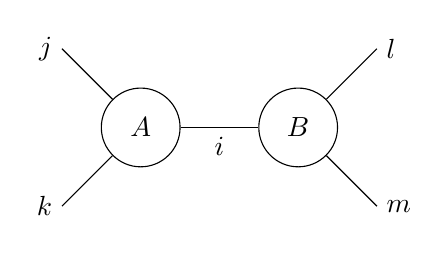
\begin{tikzpicture}
    % Nodes (Tensors)
    \node[circle, draw, minimum size=1cm] (A) at (1, 0) {$A$};
    \node[circle, draw, minimum size=1cm] (B) at (3, 0) {$B$};

    % Edges (Contractions)
    \draw[-] (A) -- (B) node[midway, below] {$i$};

    % External Legs (Free indices)
    \draw[-] (A) -- (0, 1) node[left] {$j$};
    \draw[-] (A) -- (0, -1) node[left] {$k$};
    \draw[-] (B) -- (4, 1) node[right] {$l$};
    \draw[-] (B) -- (4, -1) node[right] {$m$};
\end{tikzpicture}
\caption{A three-dimensional tensor $T_{p,q,r}$ and a tensor network of two tensors $A$, $B$ with shared index $i$.}
\label{fig:tensor_network}
\end{center}
\end{figure}

\noindent In Figure \ref{fig:tensor_network} one can see a tensor network representing the tensor contraction 
$$
C_{jklm} = \sum_{i} A_{jki} B_{ilm}.
$$

\section{Einstein Summation}
The modern Einstein summation convention is a notation used in tensor calculus that simplifies mathematical expressions. The original convention consists of eliminating the need to explicitly write summation signs by implicitly contracting all indices that are repeated in the input term. \\
In the example above, the tensor contraction would be represented as
$$C_{jklm} = A_{jki} B_{ilm} ,$$
\noindent where the index $i$ is summed over because it appears in the index sets of both $A$ and $B$.\\
This idea is extended in the modern Einstein summation convention by contracting all indices that do not appear in the output term. In modern Einstein summation, our example can be written as
$$A_{jki} B_{ilm} \rightarrow C_{jklm}.$$

This extension leads to an even more powerful formalism. By stating explicitly the indices and their order in the output tensor, we can also express other tensor operations as transpositions, dot products, traces, and outer products in this concise manner.
For example, the expression
$$A_{jki} B_{ilm} \rightarrow C_{klj}$$
means contracting the tensors via the index $i$, taking the result and summing over the axis $m$ (since the index $m$ does not appear in the output tensor) and transposing the tensor to $ C_{klj}$. \\

\noindent When using common Einstein summation APIs such as Numpy~\cite{Numpy} or PyTorch~\cite{PyTorch}, the equation is expressed by stating simply the input and output indices as a format string. The format string for our last example would be
$$jki, ilm \rightarrow klj.$$

\noindent In the following, we will refer to the Einstein summation convention as ``einsum'' and use the representation as a format string with the output tensor explicitly marked by an arrow.
